\chapter{Subjective Timbre Evaluation}
\label{chap:TimbreEvaluation}
	\todo{Come up with a better name for this chapter.}

\section{Introduction}
\label{sec:TimbreEvaluation-Introduction}
	In order to manipulate the perceptual characteristics of a sound it is necessary to know the relationships between
	low level audio features and semantic descriptions. In Chapter \ref{chap:Timbre} several different methods for
	obtaining this information were discussed.  In this chapter a new method of collecting semantically annotated audio
	feature data is presented (Section \ref{sec:TimbreEvaluation-DAWBasedTimbreEvaluation}). Data gathered using this
	method is then analysed, producing a list of semantic descriptors and the low level audio features which contribute
	to them (Section \ref{sec:TimbreEvaluation-Analysis}).

\section{Production Environment Timbre Evaluation} % this name will probably change
\label{sec:TimbreEvaluation-DAWBasedTimbreEvaluation}
	The perceptual listening test methodologies discussed in Section \ref{sec:Timbre-ListeningTests} rely on the
	participants performing a certain set of tasks. While this structure helps to reduce the number of variables in an
	experiment it does not necessarily reflect the way audio is treated in a production environment.

	A new methodology has been developed in which the analysis of timbre is introduced into a typical music production
	workflow causing minimal interruption to the producer. This methodology aims to answer the question "What terms do
	music producers use to describe the timbral transformations they apply to audio during the creation of music?". 

	This section will detail what the typical production workflow is and how semantic information can be gathered.

	\subsection{Music Production Workflow}
	\label{sec:TimbreEvaluation-DAWBasedTimbreEvaluation-Workflow}
		\todo{Find some references for this section. Probably mixing engineers handbook or something.}

		The music production workflow has four main stages:

		\begin{itemize}
			\item Recording
			\item Editing
			\item Mixing
			\item Mastering
		\end{itemize}

		At every stage of this process semantic descriptors are often used to communicate the desired timbral
		qualities of the audio. For instance one my ask that a certain microphone be used because of the `warmth' it
		adds to the recorded sound. During the mixing and mastering stages audio processing effects are applied to
		shape the timbre further.  These stages will be the focus of this section as the aim of this thesis is to
		improve the intuitiveness of these effects.

		Historically audio effects were pieces of electronic hardware through which an audio signal is passed.
		Modern music production techniques utilise Digital Audio Workstation (DAW) software. This software enables
		users to record, edit and mix multiple tracks of audio using a computer. 
		
	\subsection{Analysis of Timbre Inside the DAW}
	\label{sec:TimbreEvaluation-DAWBasedTimbreEvaluation-InDAW}
		An ideal way to collect timbral information during music production would be to have the DAW analyse the
		audio tracks used and production techniques applied. Information which could be gathered directly from the
		DAW, with no extra input from the user, includes:

		\begin{itemize}
			\item Information about the audio processing chain:
			\begin{itemize}
				\item The effects applied to each track.
				\item The order in which these effects are applied.
				\item The parameter settings of these effects.
			\end{itemize}

			\item Features of the audio signal at every stage in the processing chain.
		\end{itemize}

		Additional information can be gathered by prompting the user for input:

		\begin{itemize}
			\item The genre of music being produced.
			\item The content of the separate audio tracks (what instruments etc.).
			\item Semantic terms which describe the timbral transformations applied by each audio
			      effect.
		\end{itemize}

		Achieving this would require the creation of a new DAW. This would be impractical for the current research.
		DAWs are very comprehensive software packages which perform many more tasks than the application of effects
		to audio (project management, audio editing functionality etc.). A lot of effort would be expended in
		implementing these features before any timbral data could be collected.  Music producers also tend to have a
		preferred DAW with which they work most fluidly. Convincing producers to use a new DAW, for the purposes of
		research, would be a difficult task.

		Third party developers can produce extensions to DAWs known as plug-ins. Plug-Ins provide additional audio
		processing functionality to the DAW environment. They can optionally expose their own parameters which users
		can adjust to achieve their desired effect. There are several different formats in which audio plug-ins can
		be distributed (VST, AU etc.). Most of the commonly used DAWs support plug-ins in one or more of these
		formats.

		Audio plug-ins provide a good platform to allow producers to provide semantic terms and audio feature
		information from within their preferred DAW. As part of this research a suite of audio plug-ins which
		extract this information have been developed. They have been released under the title Semantic Audio Feature
		Extraction (SAFE) Plug-Ins.

	\subsection{SAFE Plug-Ins}
	\label{sec:TimbreEvaluation-DAWBasedTimbreEvaluation-SAFE}
		The SAFE plug-ins consist of four commonly used audio effects: Equaliser, Distortion, Compressor and Reverb.
		As part of the plug-ins's interface the user has the option to save semantic terms. The interface for the
		SAFE Distortion is shown in Figure \ref{fig:SAFE-Distortion}. Upon saving terms the plug-in will analyse the
		audio at its inputs and outputs. When the analysis is completed the results are stored, containing:

		\begin{itemize}
			\item The users description of the timbre.
			\item The plug-in's current parameter settings.
			\item The features of the audio before and after processing.
			\item Some additional data about the user and the track being worked on.
			\begin{itemize}
				\item The genre.
				\item The instrument.
				\item The users age.
				\item The users location.
				\item The users primary language.
				\item The number of year experience the user has in music production.
			\end{itemize}
		\end{itemize}

		\begin{figure}[h!]
			\centering
			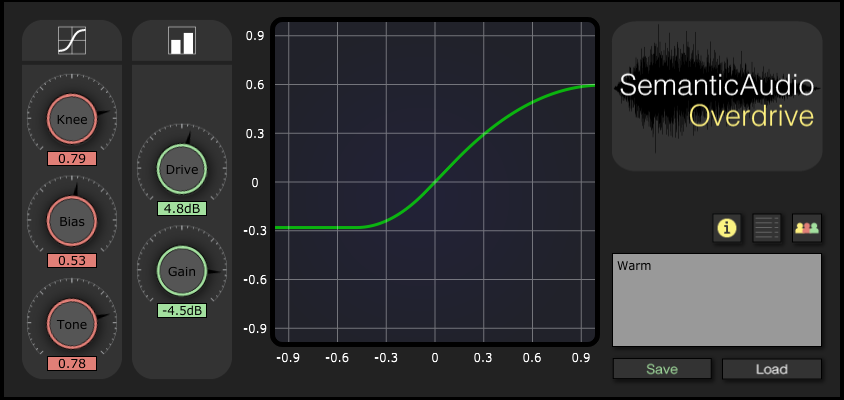
\includegraphics[width=0.8\textwidth]{chapter4/Images/SAFEDistortion.png}
			\caption{The Interface for the SAFE Distortion Plug-In}
			\label{fig:SAFE-Distortion}
		\end{figure}

		The LibXtract library \citep{bullock2007libxtract} is used in the analysis of the audio. Every scalar
		feature available within LibXtract is calculated along with the MFCCs and Bark Band Coefficients. In total
		five seconds of audio is analysed in frames of 4096 samples each.

		\note{List the features!}

		\note{Why 4096 samples? The real reason is because LibXtract works better that way. Will that cut the
		mustard?}

		One disadvantage in using plug-ins is that they cannot gather information about the processing chain they
		may be a part of. The timbral transformation the user is describing may be the result of several effects
		working together. This can be mitigated somewhat by asking users to describe only the effect the plug-in in
		question is providing.

		The SAFE plug-ins suffer from the same issues other distributed tests do. The researcher forfeits control
		over the listening environment in order to gather results from a much larger sample of people. In fact they
		provide even lest control than methodologies like that used in the Social EQ project
		\citep{cartwright2013socialeq} in that the choice of audio samples being used is decided by the test
		subject. 

	\subsection{SAFE Ontology}
	\label{sec:TimbreEvaluation-DAWBasedTimbreEvaluation-SAFEOntology}
		\note{Really not sure how well this fits in here. Do we needs a section explaining RDF and such? Where would
		that go?}

		The data collected using the SAFE plug-ins is stored as RDF triples using the SAFE ontology.  The SAFE
		Ontology was designed to describe the semantics relating to the application of an audio effect and the
		statistical audio features of the signals involved. It acts as an extension to the Audio Effects Ontology
		\citep{wilmering2013the}, introducing additional concepts for the description of semantic data.  This
		additional data can be separated into three groups:

		\begin{itemize}
			\item Metadata describing the application of the effect.
			\item Audio feature data for the input and output signals.
			\item Provenance of the data.
		\end{itemize}

		Each entry in the SAFE dataset is described using the \emph{studio:Transform} concept, applying
		some semantic transformation on a set of input signals to produce a set of output signals. The structure of
		this data is shown in Figure \ref{fig:TransformGraph}.

		\begin{figure}[h!]
			\centering
			\begin{tikzpicture}[->,>=stealth',node distance=3cm,every node/.style={scale=0.75}]
				\tikzstyle{object} = [style=ellipse]

				\node[object, fill=blue] (transform) {studio:Transform};
				\node[object, fill=green] (signal) [below left of=transform] {mo:Signal};
				\node[object, fill=orange] (descriptor) [above of=transform] {safe:DescriptorItem};
				\node[object, fill=orange] (metadata) [below right of=transform] {safe:MetadataItem};
				\node[object, fill=pink] (device) [above right=1.3cm and 0.6cm of transform] {afx:Device};
				\node[object, fill=pink] (state) [above left=1.3cm and 0.6cm of transform] {afx:State};
				\node[object, fill=gray] (harsh) [above=1cm of descriptor] {"Harsh"};

				\path (transform) edge [bend left] node [right, overlay] {prov:used} (signal)
				      edge [bend right] node [left, overlay] {prov:generated} (signal)
				      edge node [right, overlay] {safe:descriptor} (descriptor)
				      edge [bend left] node [right, overlay] {safe:metadata} (metadata)
				      edge [bend right] node [right, overlay] {studio:effect} (device)
				      edge [bend left] node [left, overlay] {afx:state} (state)
				      (signal) edge [bend right] node [below, overlay] {safe:metadata} (metadata)
				      (descriptor) edge node [right, overlay] {rdfs:comment} (harsh);
			\end{tikzpicture}
			\caption{The structure used to describe the application of an audio effect.}
			\label{fig:TransformGraph}
		\end{figure}

		Here, users provide a term, or series of terms, to describe the transform applied by the audio effect in its
		current state. This should describe the perceived difference between the output and input signals. In the
		SAFE Ontology this is modelled through the \emph{safe:DescriptorItem} concept which provides a semantic
		description for each transform. Metadata items are used to provide details about the application domain of
		the effect, where each metadata item describes one property of an object, the property being identified
		using an \emph{rdfs:label} and the description provided using an \emph{rdfs:comment}. Each object described
		by a metadata item has its own set of properties, ``genre'' and ``instrument'' metadata tags for example,
		describe an audio signal, while ``location'' metadata tags describe a transform.

		The analysis of audio signals is described using the concept \emph{safe:FeatureExtractionTransform}, similar
		to a \emph{studio:Transform} but taking an audio signal as input and producing feature values at the output,
		as shown in Figure \ref{fig:ExtractionGraph}.

		\begin{figure}[h!]
			\centering
			\begin{tikzpicture}[->,>=stealth',node distance=3cm,every node/.style={scale=0.75}]
				\tikzstyle{object} = [style=ellipse]

				\node[object, fill=orange] (extraction) {safe:FeatureExtractionTransform};
				\node[object, fill=gray] (feature) [above of=extraction] {"Spectral Centroid"};
				\node[object, fill=gray] (frameSize) [above left of=extraction] {"4096"};
				\node[object, fill=gray] (stepSize) [above right of=extraction] {"1024"};
				\node[object, fill=green] (signal) [below left of=extraction] {mo:Signal};
				\node[object, fill=purple] (event) [below right of=extraction] {event:Event};
				\node[object, fill=yellow] (interval) [below=1cm of signal] {tl:Interval};
				\node[object, fill=yellow] (instant) [below=1cm of event] {tl:Instant};
				\node[object, fill=yellow] (timeline) [below right of=interval] {tl:TimeLine};
				\node[object, fill=gray] (value) [below right=0.2cm and 0.6cm of event] {"2543.4"};
				\node[object, fill=gray] (time) [below right=0.2cm and 0.6cm of instant] {"4048"};

				\path (extraction) edge [bend left] node [left, overlay] {safe:frameSize} (frameSize)
				      edge [bend right] node [right, overlay] {safe:stepSize} (stepSize)
				      edge node [right, overlay] {rdfs:label} (feature)
				      edge [bend right] node [left, overlay] {prov:used} (signal)
				      (signal) edge node [left, overlay] {mo:time} (interval)
				      (event) edge node [left, overlay] {event:time} (instant)
				      edge [bend right] node [right, overlay] {prov:wasGeneratedBy} (extraction)
				      edge node [above right, overlay] {af:feature} (value)
				      (interval) edge [bend right] node [left, overlay] {tl:onTimeLine} (timeline)
				      (instant) edge [bend left] node [right, overlay] {tl:onTimeLine} (timeline)
				      edge node [above right, overlay] {tl:at} (time);

			\end{tikzpicture}
			\caption{The structure used to describe the features of an audio signal.}
			\label{fig:ExtractionGraph}
		\end{figure}

		Here, The SAFE Ontology makes extensive use of the Provenance Ontology to identify the origins of the data.
		Each element of data constitutes a \emph{prov:Entity} which was generated by a \emph{prov:Activity}. These
		\emph{prov:Activity} nodes are in turn associated with a \emph{prov:Agent} identifying the way that the data
		was produced.

		When using the SAFE plug-ins, users are required to provide a descriptor for a transform, meaning that every
		\emph{safe:DescriptorItem} node in the dataset is attributed to a particular user. Conversely, the metadata
		fields are not mandatory. In situations where a user has not filled in certain metadata fields their values
		can be predicted on the server using supervised machine learning. Using the Provenance Ontology, each
		metadata entity can be attributed to a particular agent, allowing it to understood as human or machine
		labelled. This allows queries on the dataset to request only the more reliable user-labeled data, or for
		example, compare data produced using different classification algorithms.

		The Provenance Ontology is also used to describe the algorithms that produce audio feature data. Each
		\emph{safe:FeatureExtractionTransform} node is a \emph{prov:Activity} which can be associated with a
		particular implementation of the algorithm it uses (e.g. the LibXtract \citep{bullock2007libxtract} spectral
		centroid function). Say a discrepancy was found between two implementations of a given feature extraction
		algorithm, the provenance data allows queries to filter results to remove those generated using an earlier
		or incompatible implementation. Further use of provenance describes the role of a user in the application of
		a transform. Storage of this data allows the simple retrieval of all transforms associated with a particular
		user, allowing users to maintain personal libraries of semantic presets amongst the entire SAFE dataset.

\section{Analysis}
\label{sec:TimbreEvaluation-Analysis}
	In this section the data collected using the SAFE plug-ins is analysed. For the purposes of this study only the data
	from the distortion and equaliser plug-ins is used as these effects best represent the timbral transformations which
	can be applied using harmonic excitation. The distortion showing the effects of introducing new spectral content and
	the equaliser showing the effects of manipulating the existing spectral content.

	Firstly, the terms used to describe transformations using each plug-in are investigated (Section
	\ref{sec:TimbreEvaluation-Analysis-TermUsage}). This provides insight into the language used to describe audio in
	the production environment, also showing what terms are shared across processing techniques and those which are
	reserved for particular effect. Secondly, clustering techniques are used in order to group these terms into those
	which describe similar audio signals / transformations, finding terms which are synonymous when used to describe
	timbre (Section \ref{sec:TimbreEvaluation-Analysis-TermClustering}). Finally, timbre spaces are constructed using
	MDS in order to find the most salient audio features which contribute to the differences in timbral description.

	\subsection{Term Usage}
	\label{sec:TimbreEvaluation-Analysis-TermUsage}
		Tables \ref{tab:DistortionTerms} and \ref{tab:EqualiserTerms} show the most commonly used terms used to
		describe transforms applied by the distortion and equaliser respectively.

		\begin{table}[h!]
			\centering
			\begin{tabular}{|c|c|}
				\hline
				\bf{Term} & \bf{Frequency} \\
				\hline
				\hline
				warm & 21 \\
				\hline
				crunch & 16 \\
				\hline
				crunchy & 10 \\
				\hline
				fuzz & 9 \\
				\hline
				creamy & 6 \\
				\hline
			\end{tabular}
			\qquad
			\begin{tabular}{|c|c|}
				\hline
				\bf{Term} & \bf{Frequency} \\
				\hline
				\hline
				fuzzy & 6 \\
				\hline
				bright & 5 \\
				\hline
				harsh & 4 \\
				\hline
				raspy & 4 \\
				\hline
				smooth & 3 \\
				\hline
			\end{tabular}
			\caption{Most Commonly Used Terms from the Distortion.}
			\label{tab:DistortionTerms}
		\end{table}

		\begin{table}[h!]
			\centering
			\begin{tabular}{|c|c|}
				\hline
				\bf{Term} & \bf{Frequency} \\
				\hline
				\hline
				warm & 437 \\
				\hline
				bright & 408 \\
				\hline
				clear & 17 \\
				\hline
				thin & 11 \\
				\hline
				airy & 9 \\
				\hline
			\end{tabular}
			\qquad
			\begin{tabular}{|c|c|}
				\hline
				\bf{Term} & \bf{Frequency} \\
				\hline
				\hline
				boomy & 8 \\
				\hline
				air & 7 \\
				\hline
				brighter & 6 \\
				\hline
				deep & 6 \\
				\hline
				full & 6 \\
				\hline
			\end{tabular}
			\qquad
			\begin{tabular}{|c|c|}
				\hline
				\bf{Term} & \bf{Frequency} \\
				\hline
				\hline
				tinny & 6 \\
				\hline
				muddy & 5 \\
				\hline
				boxy & 4 \\
				\hline
				harsh & 4 \\
				\hline
				box & 3 \\
				\hline
			\end{tabular}
			\caption{Most Commonly Used Terms from the Equaliser.}
			\label{tab:EqualiserTerms}
		\end{table}

		\note
		{
			Should we mention how `warm' and `bright' from the EQ have so many instances because they were part
			of an experiment?
		}

		The terms `warm' and `bright' have been used to describe transformations applied using both the distortion
		and the equaliser effects, suggesting that the timbral characteristics these terms describe can be
		manipulated using either effect. Other descriptors are only used to describe transformations applied using a
		specific effect, suggesting that a unique property of that effect produces tat timbral result. For example
		the term `crunch' is only used to in relation to the distortion effect.

		Several descriptors in the dataset are derived from the same root word with the addition of suffixes such as
		`y' or `er' (e.g. `crunch' and `crunchy' or `bright' and `brighter'). It is assumed that the addition of
		such suffixes has no effect over how a term is used to describe timbre. As such a stemming algorithm
		\citep{porter1980an} is used in order to reduce all descriptors in the dataset to their root words.
		Additional processing is required after stemming so that all descriptors with the same root can be combined.
		The Porter stemming algorithm replaces the letter y at the end of a word with the letter i, for this
		analysis these tailing i's are removed so that terms such as `fuzz' and `fuzzy' are reduced to the same
		root. In some cases the output after this  must be further reduced, for example the term `muddy' is
		reduced to `mudd' which must have the tailing d removed to give the correct root `mud'.

		After stemming we are left with eight descriptors from the distortion (`warm', `crunch', `fuzz', `cream',
		`bright', `harsh', `rasp' and `smooth') and twelve descriptors from the equaliser (`warm', `bright',
		`clear', `thin', `air', `boom', `deep', `full', `tin', `mud', `box' and `harsh').

	\subsection{Term Clustering}
	\label{sec:TimbreEvaluation-Analysis-TermClustering}
		Each of the terms arrived at, after stemming, in Section \ref{sec:TimbreEvaluation-Analysis-TermClustering}
		can be described by their position in a multi dimensional audio feature space. Each dimension of this space
		corresponds to one of the audio features extracted by the SAFE plug-ins. The coordinates of each term are
		calculated as the mean audio features across each transform described by that term. Two separate feature
		spaces are constructed, one in which the audio features of the processed signal are used and one in which
		the difference between features of the output and input signal are used. These two spaces can be compared to
		determine whether certain descriptors are mostly used to describe a transform (e.g. an increase in
		inharmonicity) or are used to describe an output signal (e.g. a signal with a spectral centroid between 4
		and 8kHz).

		\begin{figure}[h!]
			\centering
			\subfloat[Processed Features]
			{
				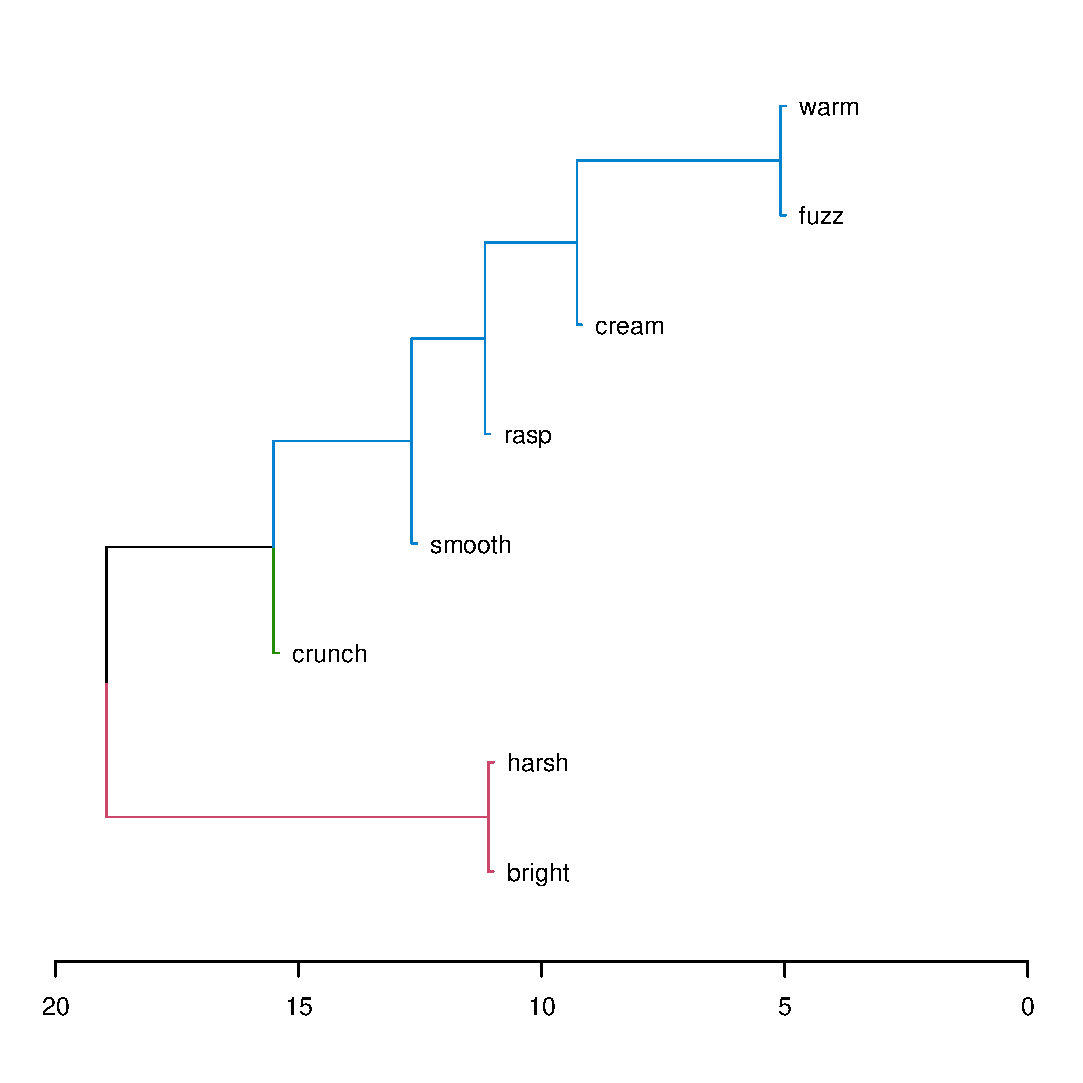
\includegraphics[width=0.45\textwidth]{chapter4/Images/DistortionProcessedClusters.eps}
				\label{fig:DistortionProcessedClusters}
			}
			\qquad
			\subfloat[Feature Differences]
			{
				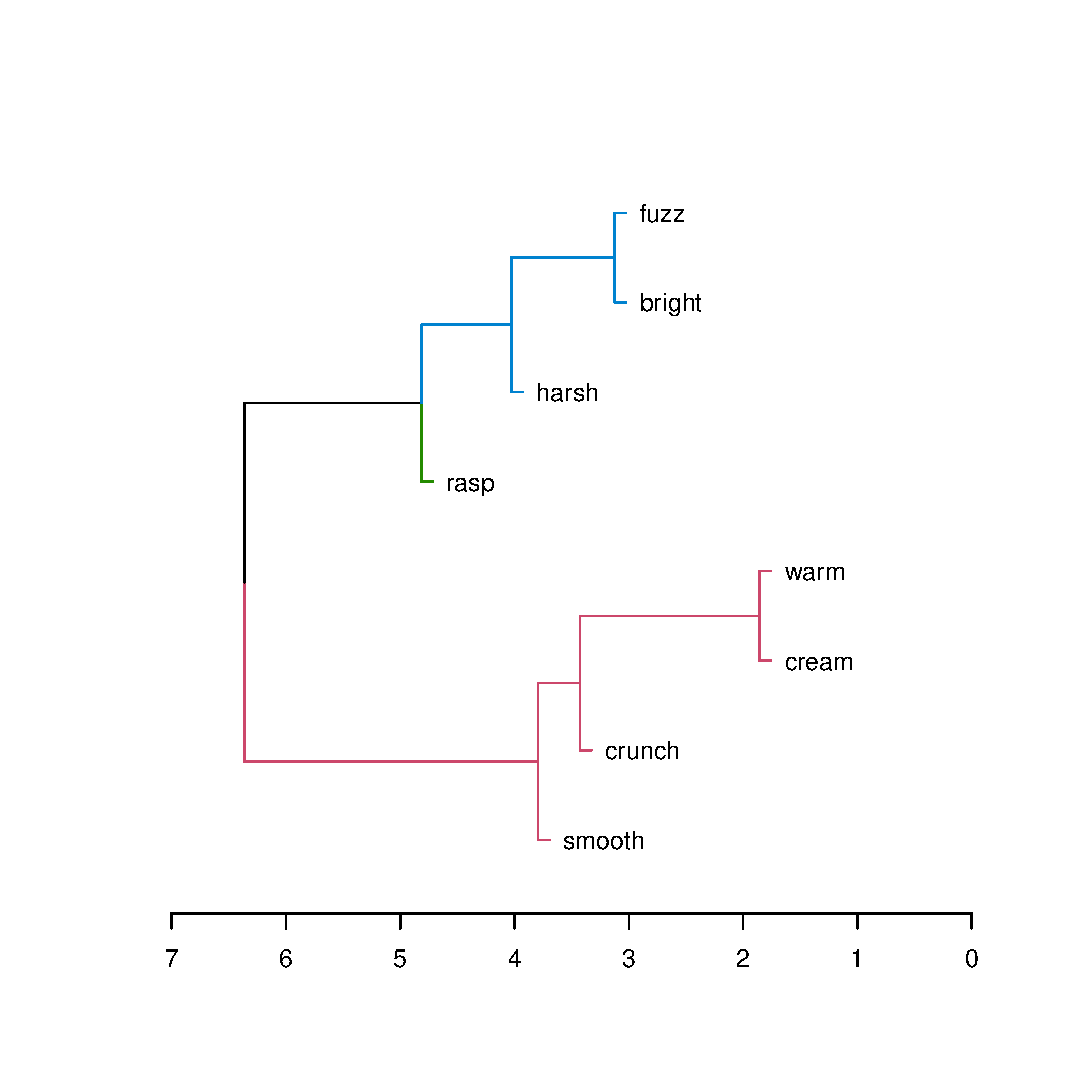
\includegraphics[width=0.45\textwidth]{chapter4/Images/DistortionDifferenceClusters.eps}
				\label{fig:DistortionDifferenceClusters}
			}
			\caption{Clustering of descriptors from the Distortion}
			\label{fig:DistortionClusters}
		\end{figure}

		\begin{figure}[h!]
			\centering
			\subfloat[Processed Features]
			{
				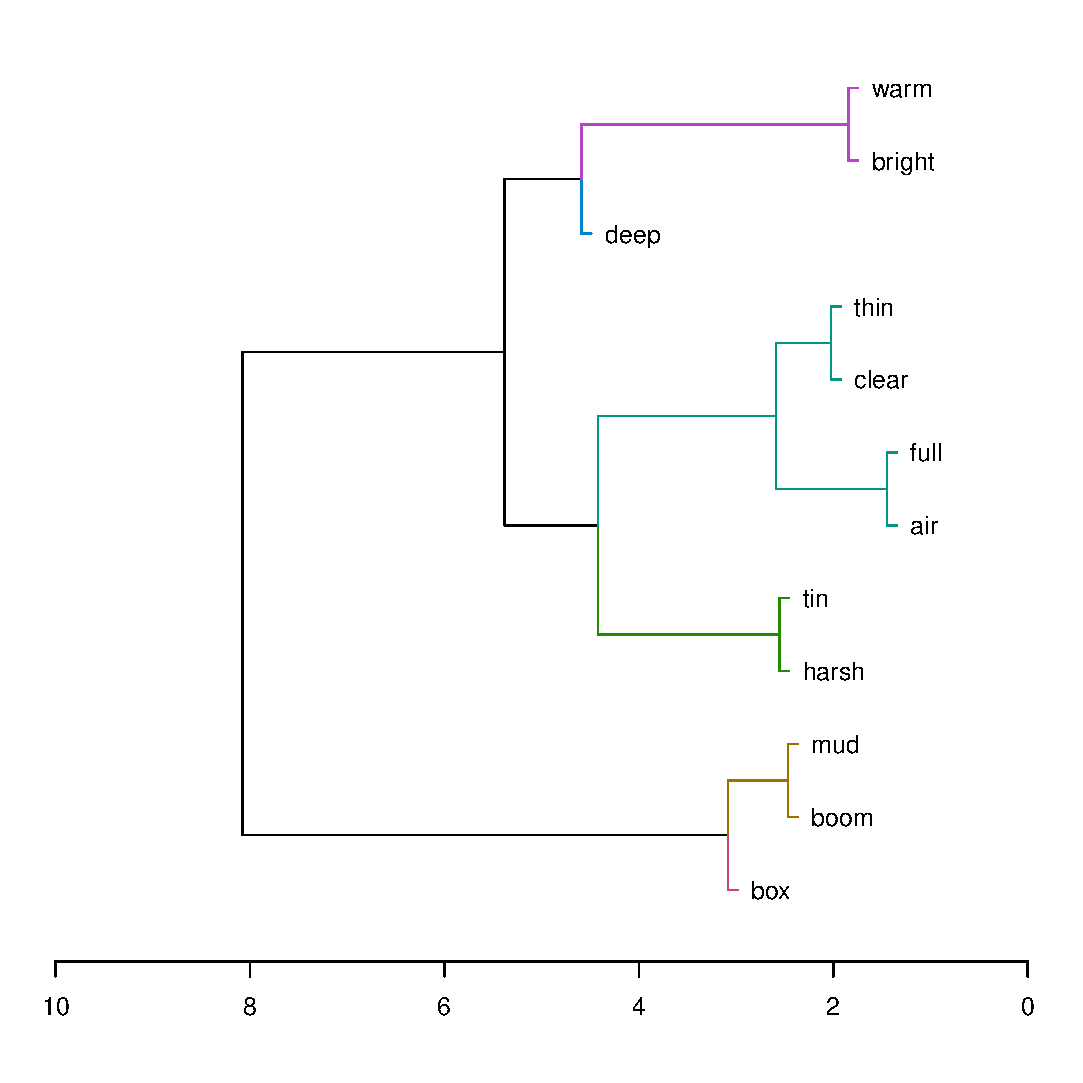
\includegraphics[width=0.45\textwidth]{chapter4/Images/EqualiserProcessedClusters.eps}
				\label{fig:EqualiserProcessedClusters}
			}
			\qquad
			\subfloat[Feature Differences]
			{
				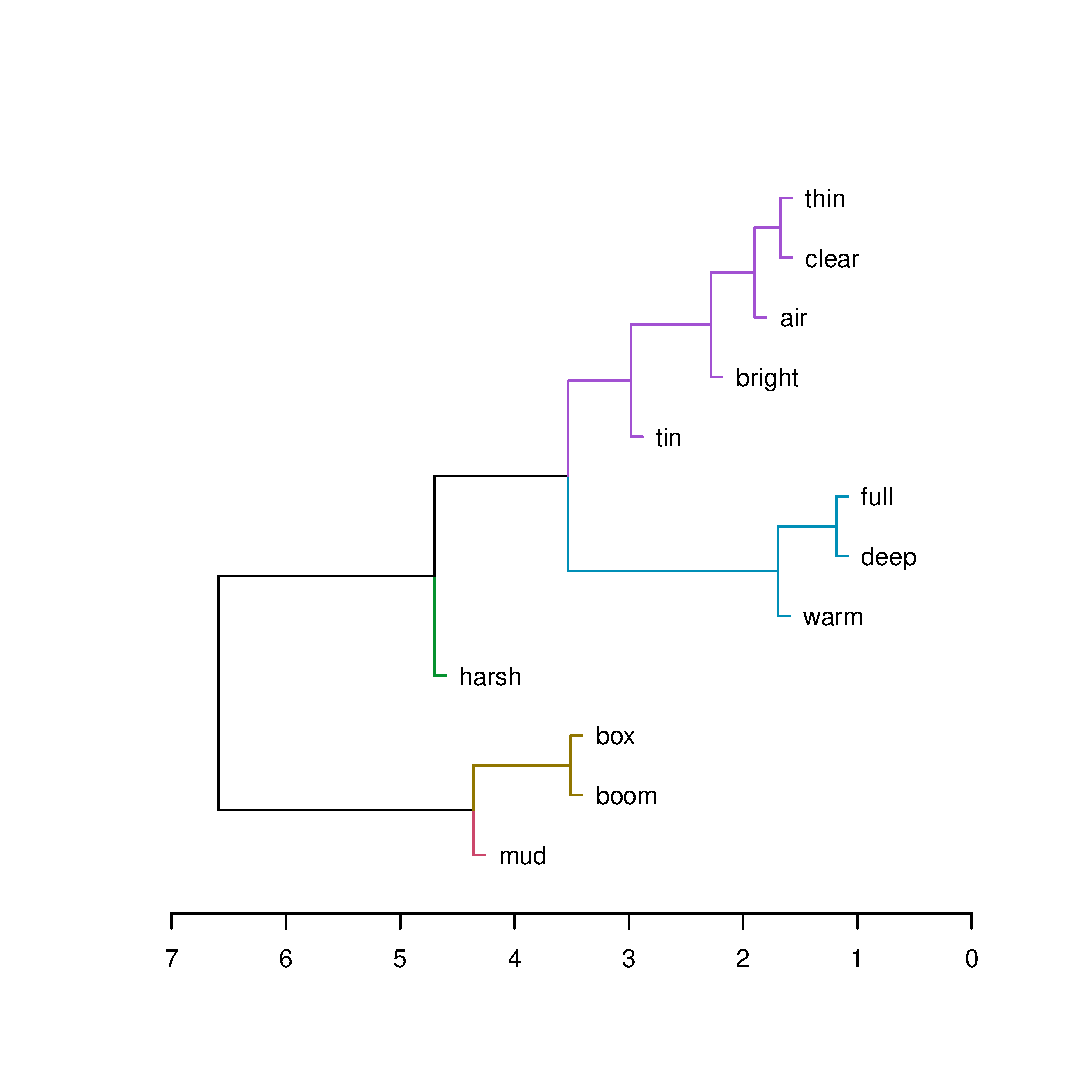
\includegraphics[width=0.45\textwidth]{chapter4/Images/EqualiserDifferenceClusters.eps}
				\label{fig:EqualiserDifferenceClusters}
			}
			\caption{Clustering of descriptors from the Equaliser}
			\label{fig:EqualiserClusters}
		\end{figure}

	\subsection{Timbre Spaces}
	\label{sec:TImbreEvaluation-Analysis-TimbreSpaces}

		\begin{figure}[h!]
			\centering
			\subfloat[Individual Transforms]
			{
				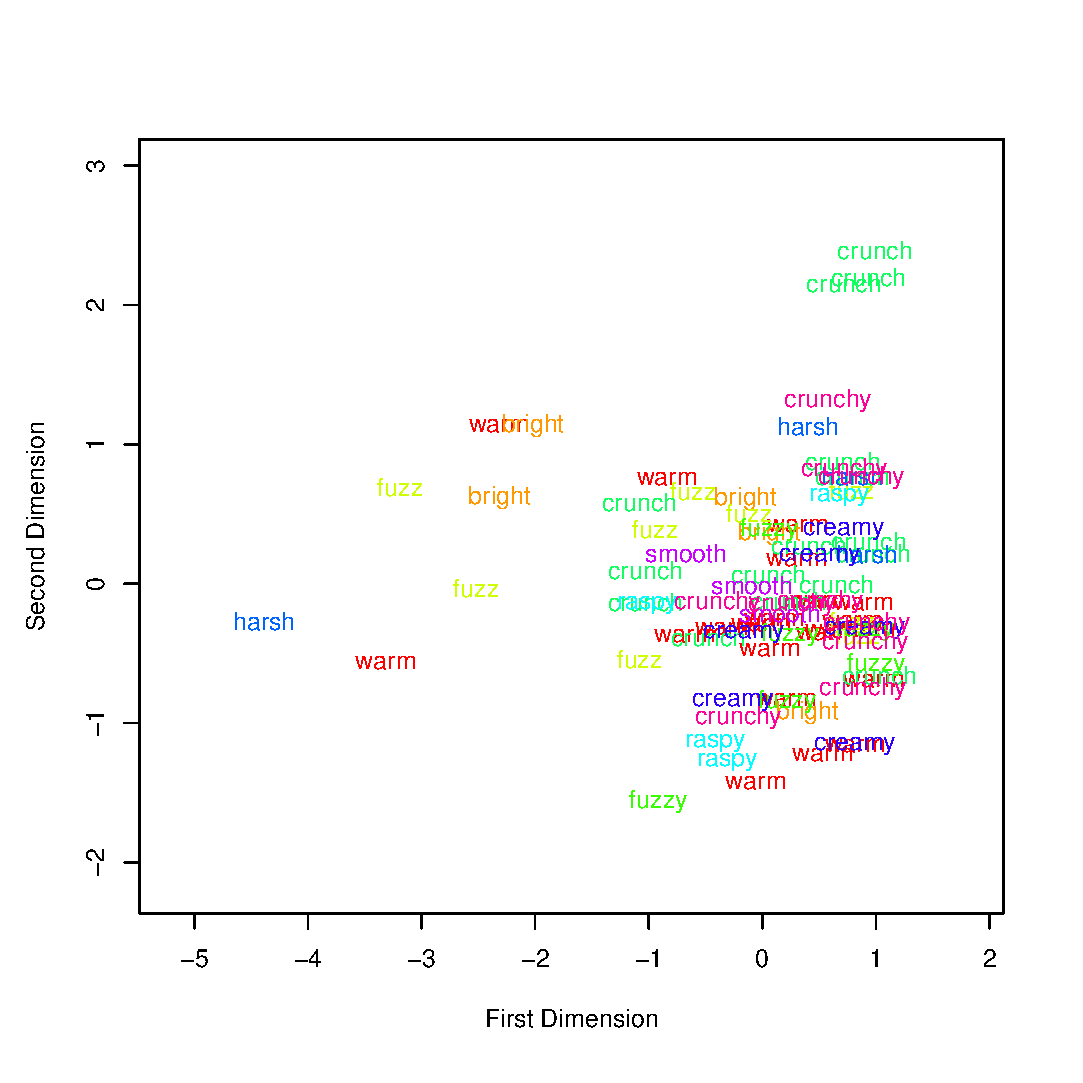
\includegraphics[width=0.45\textwidth]{chapter4/Images/DistortionProcessedMDS.eps}
				\label{fig:DistortionProcessedMDS}
			}
			\qquad
			\subfloat[Descriptor Centroids]
			{
				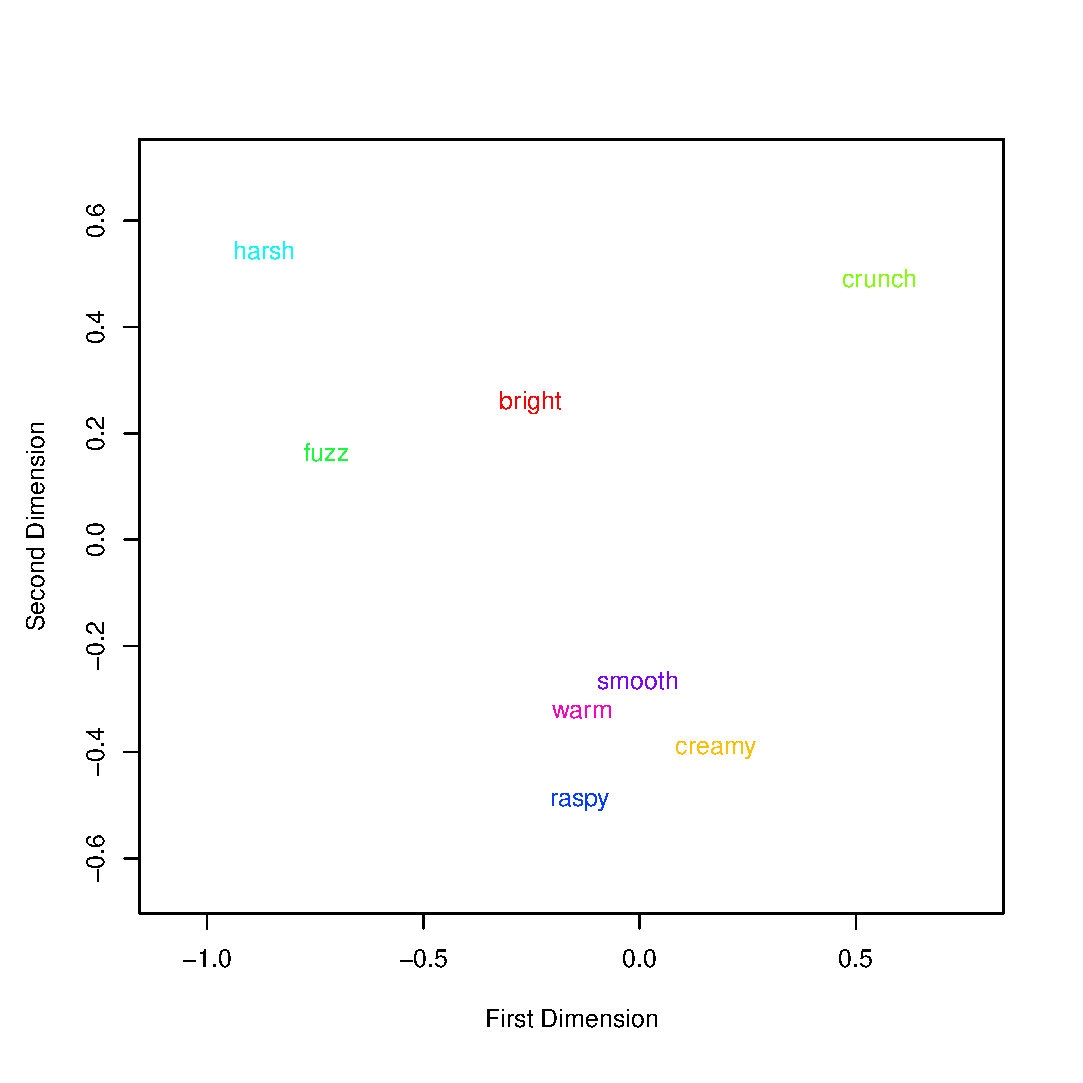
\includegraphics[width=0.45\textwidth]{chapter4/Images/DistortionProcessedCentroidsMDS.eps}
				\label{fig:DistortionProcessedCentroidsMDS}
			}
			\caption{Timbre Space for the Processed Features from the Distortion.}
			\label{fig:DistortionProcessedMDSs}
		\end{figure}

		\begin{table}[h!]
			\centering
			\begin{tabular}{|c|c|}
				\hline
				\bf{Feature} & \bf{Correlation} \\
				\hline
				\hline
				Irregularity K & -0.977 \\
				\hline
				Bark Coefficient 6 & -0.957 \\
				\hline
				Peak Irregularity K & -0.952 \\
				\hline
				Bark Coefficient 7 & -0.944 \\
				\hline
				Peak Spectral Kurtosis & -0.939 \\
				\hline
				Bark Coefficient 5 & -0.932 \\
				\hline
				Bark Coefficient 8 & -0.929 \\
				\hline
				Peak Spectral Skewness & -0.916 \\
				\hline
				Harmonic Spectral Kurtosis & -0.914 \\
				\hline
				Bark Coefficient 9 & -0.908 \\
				\hline
				Harmonic Irregularity K & -0.908 \\
				\hline
				Bark Coefficient 15 & -0.899 \\
				\hline
				Bark Coefficient 12 & -0.899 \\
				\hline
				Bark Coefficient 24 & -0.897 \\
				\hline
				Bark Coefficient 4 & -0.894 \\
				\hline
				Spectral Skewness & -0.890 \\
				\hline
				Harmonic Spectral Skewness & -0.889 \\
				\hline
				Bark Coefficient 11 & -0.877 \\
				\hline
				Bark Coefficient 17 & -0.876 \\
				\hline
				Bark Coefficient 10 & -0.871 \\
				\hline
				Bark Coefficient 13 & -0.870 \\
				\hline
				Bark Coefficient 18 & -0.866 \\
				\hline
				Bark Coefficient 14 & -0.850 \\
				\hline
				Bark Coefficient 16 & -0.844 \\
				\hline
				Bark Coefficient 19 & -0.844 \\
				\hline
				Bark Coefficient 3 & -0.833 \\
				\hline
				Bark Coefficient 23 & -0.828 \\
				\hline
				Bark Coefficient 2 & -0.819 \\
				\hline
				Standard Deviation & -0.809 \\
				\hline
				RMS Amplitude & -0.809 \\
				\hline
			\end{tabular}
			\caption{Significant Features for Dimension 1 of the Timbre Spaces Shown in Figure 
				 \ref{fig:DistortionProcessedMDSs}.}
			\label{tab:DistortionProcessedFeaturesDim1}
		\end{table}

		\begin{table}[h!]
			\centering
			\begin{tabular}{|c|c|}
				\hline
				\bf{Feature} & \bf{Correlation} \\
				\hline
				\hline
				Spectral Roll Off &  0.899 \\
				\hline
				MFCC 1 & -0.892 \\
				\hline
				Spectral Centroid &  0.880 \\
				\hline
				Spectral Slope &  0.859 \\
				\hline
				Peak Spectral Standard Deviation &  0.857 \\
				\hline
				Harmonic Spectral Standard Deviation &  0.854 \\
				\hline
				Harmonic Spectral Centroid &  0.837 \\
				\hline
				Peak Spectral Centroid &  0.835 \\
				\hline
			\end{tabular}
			\caption{Significant Features for Dimension 2 of the Timbre Spaces Shown in Figure 
				 \ref{fig:DistortionProcessedMDSs}.}
			\label{tab:DistortionProcessedFeaturesDim2}
		\end{table}

		\begin{figure}[h!]
			\centering
			\subfloat[Individual Transforms]
			{
				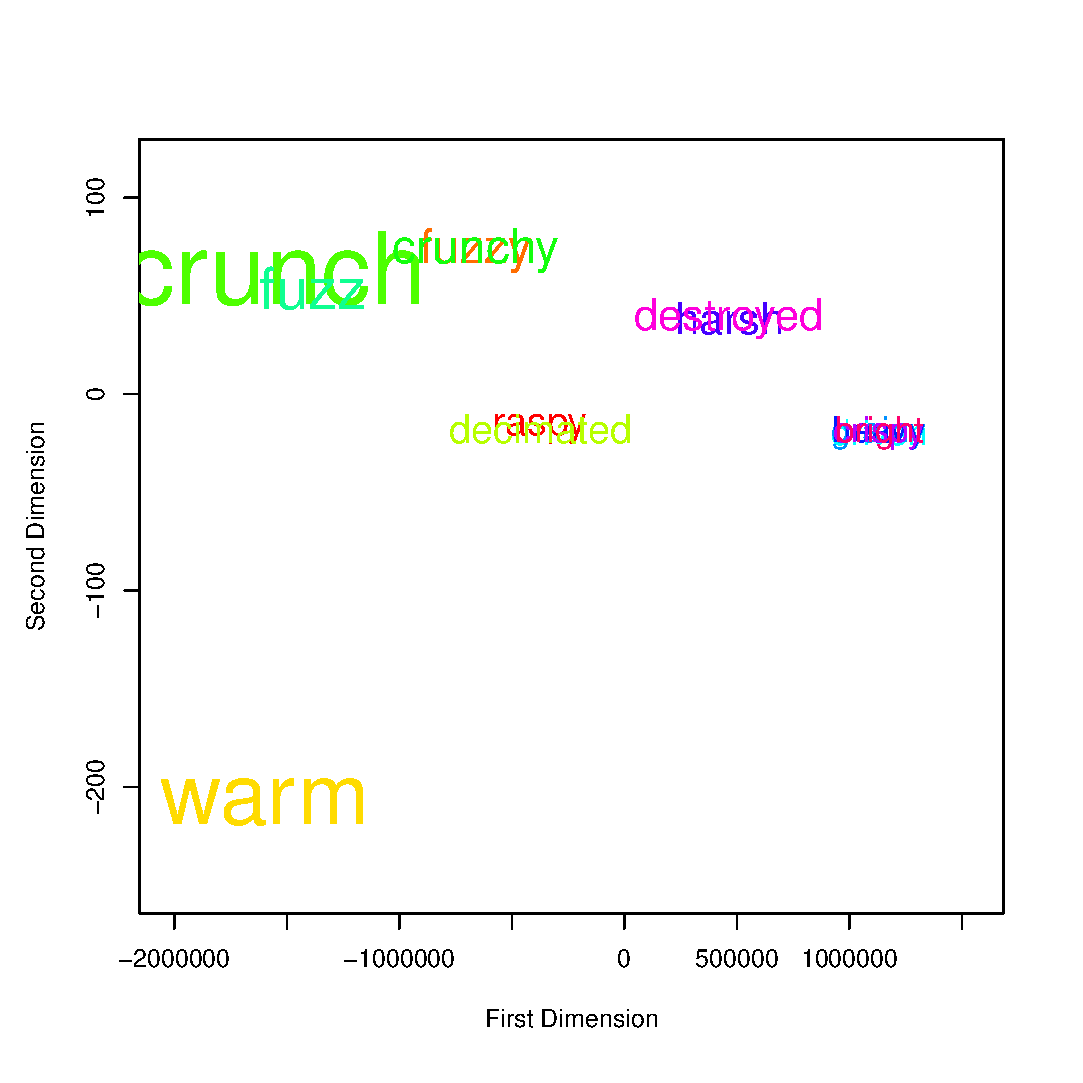
\includegraphics[width=0.45\textwidth]{chapter4/Images/DistortionDifferenceMDS.eps}
				\label{fig:DistortionDifferenceMDS}
			}
			\qquad
			\subfloat[Descriptor Centroids]
			{
				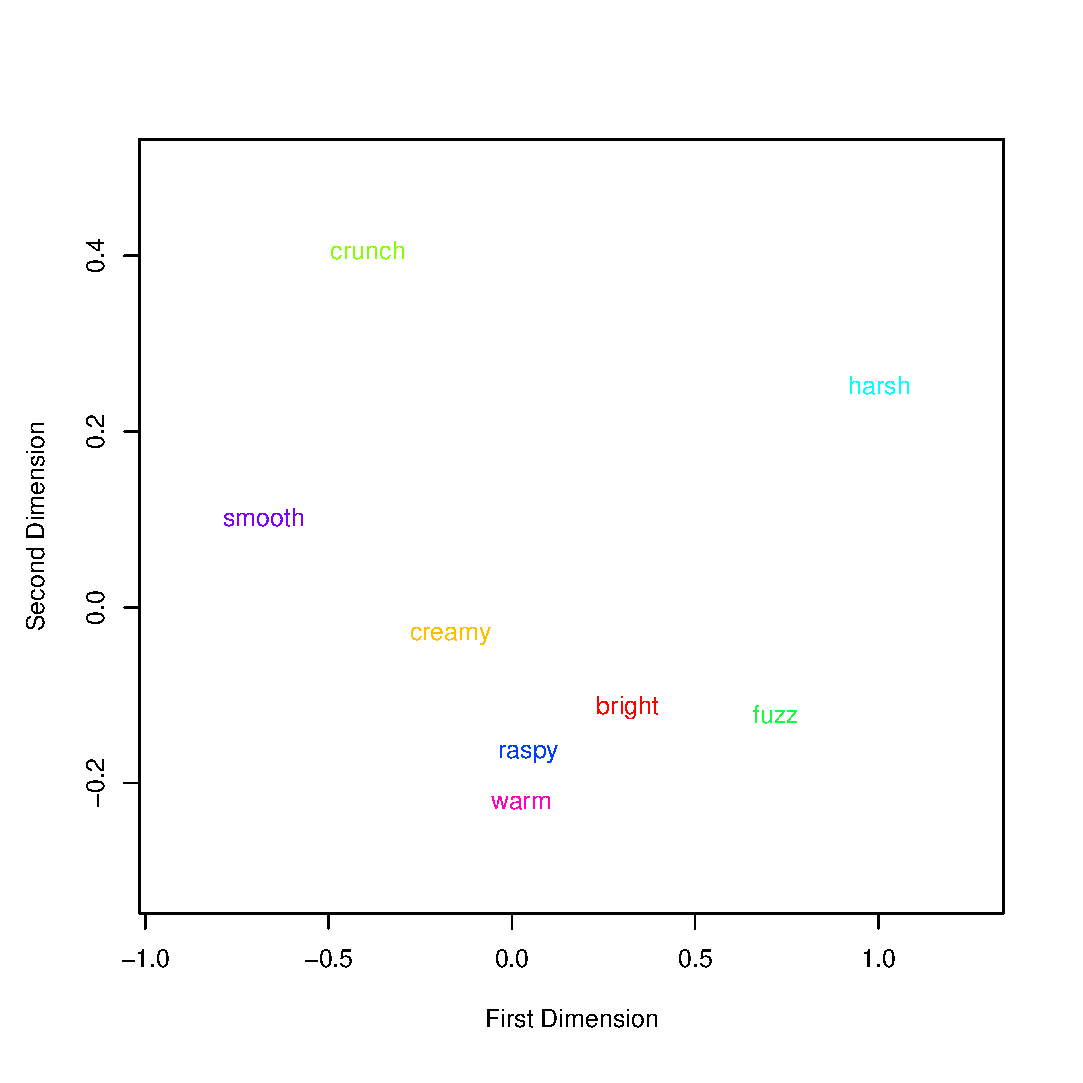
\includegraphics[width=0.45\textwidth]{chapter4/Images/DistortionDifferenceCentroidsMDS.eps}
				\label{fig:DistortionDifferenceCentroidsMDS}
			}
			\caption{Timbre Space for the Feature Differences from the Distortion.}
			\label{fig:DistortionDifferenceMDSs}
		\end{figure}

		\begin{table}[h!]
			\centering
			\begin{tabular}{|c|c|}
				\hline
				\bf{Feature} & \bf{Correlation} \\
				\hline
				\hline
				Irregularity K & 0.984 \\
				\hline
				Peak Irregularity K & 0.966 \\
				\hline
				Bark Coefficient 6 & 0.956 \\
				\hline
				Bark Coefficient 7 & 0.949 \\
				\hline
				Bark Coefficient 15 & 0.948 \\
				\hline
				Bark Coefficient 8 & 0.946 \\
				\hline
				Bark Coefficient 9 & 0.942 \\
				\hline
				Harmonic Irregularity K & 0.936 \\
				\hline
				Bark Coefficient 5 & 0.936 \\
				\hline
				Bark Coefficient 17 & 0.930 \\
				\hline
				Bark Coefficient 16 & 0.926 \\
				\hline
				Bark Coefficient 14 & 0.925 \\
				\hline
				Peak Spectral Skewness & 0.923 \\
				\hline
				Bark Coefficient 10 & 0.922 \\
				\hline
				Bark Coefficient 13 & 0.919 \\
				\hline
				Bark Coefficient 12 & 0.918 \\
				\hline
				Bark Coefficient 18 & 0.913 \\
				\hline
				Peak Spectral Kurtosis & 0.911 \\
				\hline
				Bark Coefficient 11 & 0.909 \\
				\hline
				Harmonic Spectral Skewness & 0.906 \\
				\hline
				Harmonic Spectral Kurtosis & 0.888 \\
				\hline
				Bark Coefficient 4 & 0.883 \\
				\hline
				RMS Amplitude & 0.882 \\
				\hline
				Standard Deviation & 0.882 \\
				\hline
				Bark Coefficient 19 & 0.877 \\
				\hline
				Bark Coefficient 3 & 0.854 \\
				\hline
				Spectral Skewness & 0.854 \\
				\hline
				Bark Coefficient 20 & 0.852 \\
				\hline
				Bark Coefficient 2 & 0.841 \\
				\hline
				Bark Coefficient 22 & 0.838 \\
				\hline
				Bark Coefficient 23 & 0.834 \\
				\hline
				Bark Coefficient 21 & 0.833 \\
				\hline
			\end{tabular}
			\caption{Significant Features for Dimension 1 of the Timbre Spaces Shown in Figure 
				 \ref{fig:DistortionDifferenceMDSs}.}
			\label{tab:DistortionDifferenceFeaturesDim1}
		\end{table}

		\begin{table}[h!]
			\centering
			\begin{tabular}{|c|c|}
				\hline
				\bf{Feature} & \bf{Correlation} \\
				\hline
				\hline
				Spectral Variance & -0.896 \\
				\hline
				Spectral Roll Off & -0.878 \\
				\hline
				Spectral Centroid & -0.868 \\
				\hline
				Harmonic Spectral Centroid & -0.849 \\
				\hline
				Harmonic Spectral Standard Deviation & -0.848 \\
				\hline
				Peak Spectral Centroid & -0.833 \\
				\hline
				Spectral Standard Deviation & -0.808 \\
				\hline
				Peak Spectral Variance & -0.807 \\
				\hline
				Peak Spectral Standard Deviation & -0.806 \\
				\hline
				Harmonic Spectral Variance & -0.802 \\
				\hline
			\end{tabular}
			\caption{Significant Features for Dimension 2 of the Timbre Spaces Shown in Figure 
				 \ref{fig:DistortionDifferenceMDSs}.}
			\label{tab:DistortionDifferenceFeaturesDim2}
		\end{table}

		\begin{figure}[h!]
			\centering
			\subfloat[Individual Transforms]
			{
				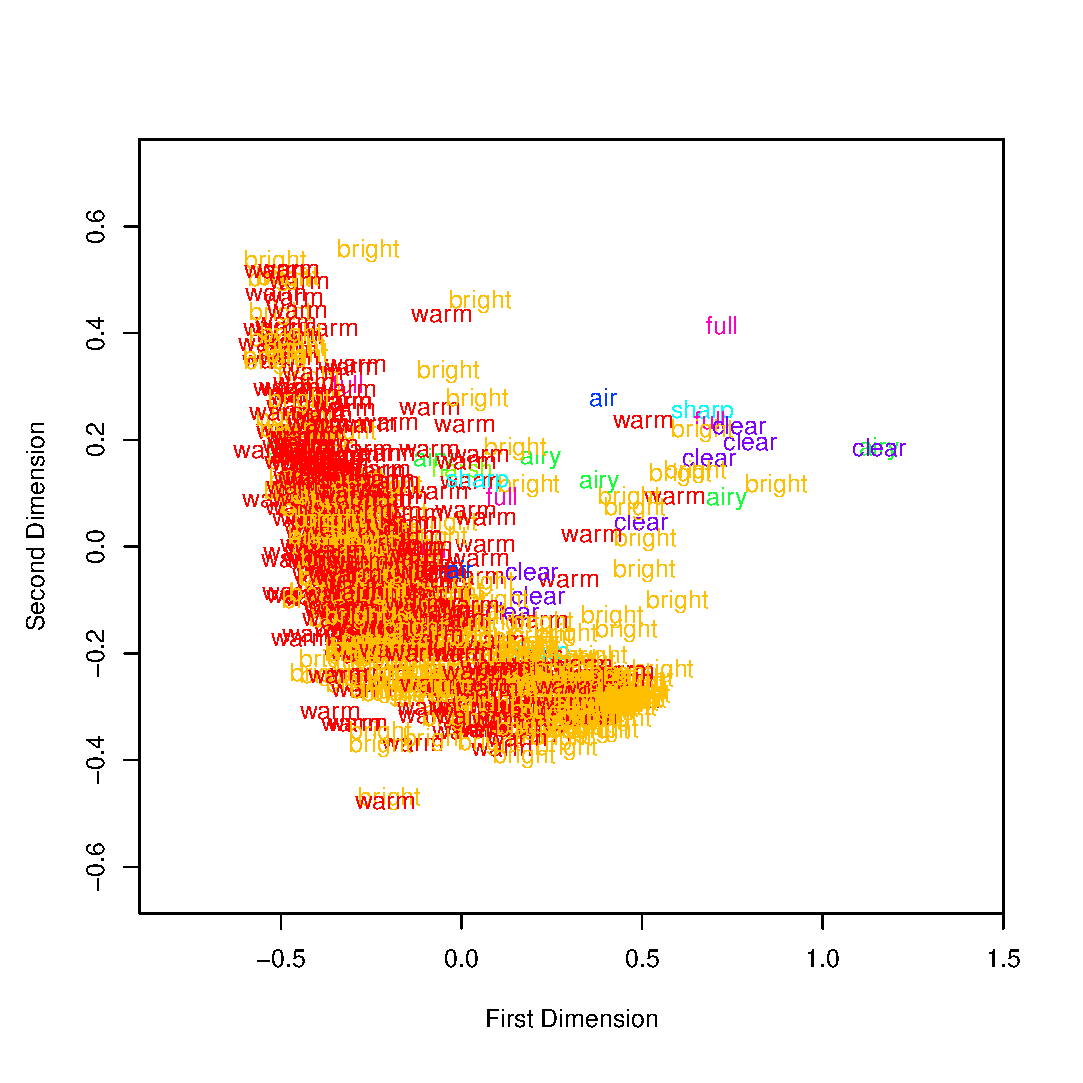
\includegraphics[width=0.45\textwidth]{chapter4/Images/EqualiserProcessedMDS.eps}
				\label{fig:EqualiserProcessedMDS}
			}
			\qquad
			\subfloat[Descriptor Centroids]
			{
				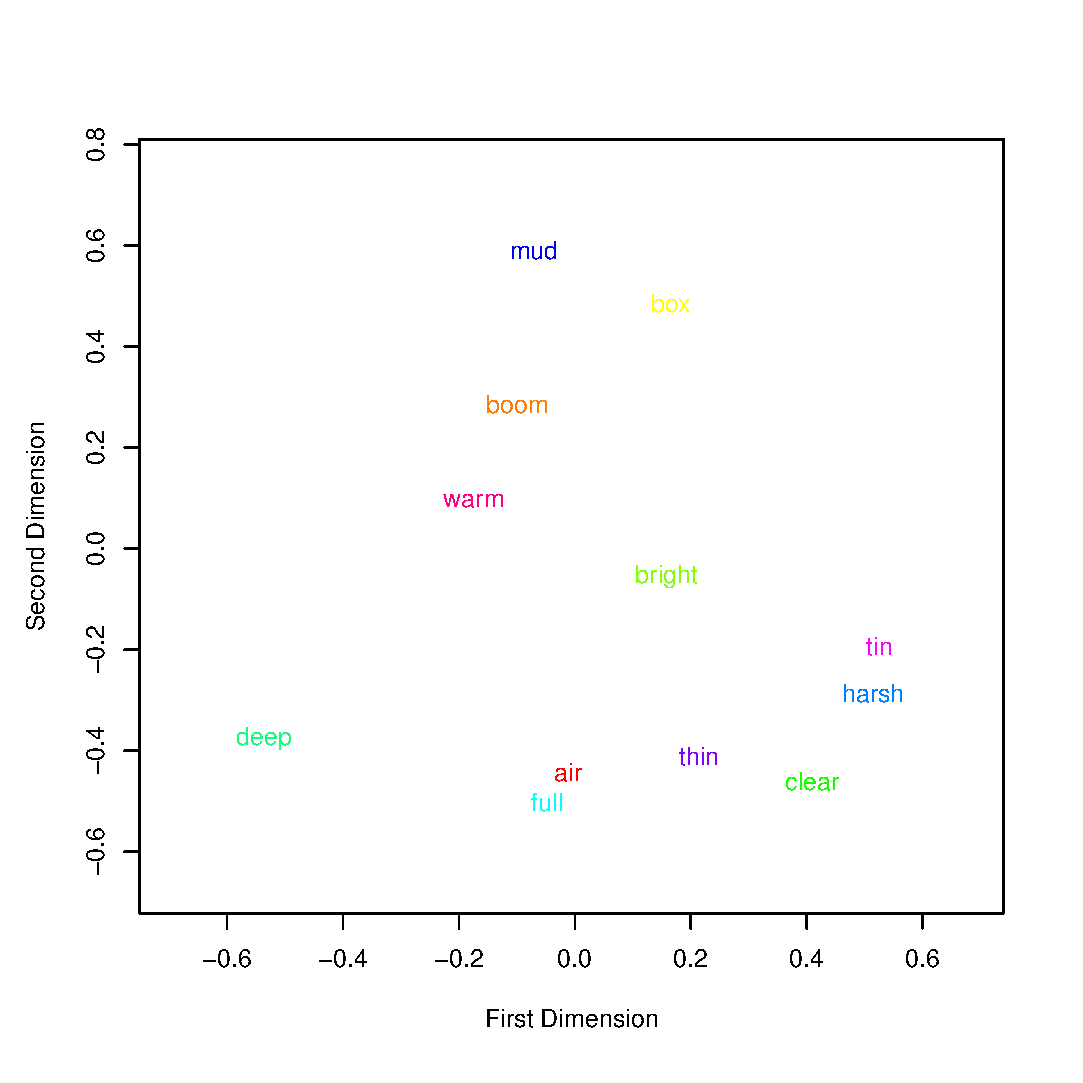
\includegraphics[width=0.45\textwidth]{chapter4/Images/EqualiserProcessedCentroidsMDS.eps}
				\label{fig:EqualiserProcessedCentroidsMDS}
			}
			\caption{Timbre Space for the Processed Features from the Equaliser.}
			\label{fig:EqualiserProcessedMDSs}
		\end{figure}

		\begin{table}[h!]
			\centering
			\begin{tabular}{|c|c|}
				\hline
				\bf{Feature} & \bf{Correlation} \\
				\hline
				\hline
				Peak Tristimulus 2 & -0.863 \\
				\hline
				Harmonic Tristimulus 2 & -0.852 \\
				\hline
				Spectral Crest & -0.842 \\
				\hline
				Harmonic Spectral Standard Deviation &  0.829 \\
				\hline
				Peak Spectral Standard Deviation &  0.826 \\
				\hline
				Peak Spectral Centroid &  0.814 \\
				\hline
				Harmonic Spectral Centroid &  0.811 \\
				\hline
			\end{tabular}
			\caption{Significant Features for Dimension 1 of the Timbre Spaces Shown in Figure 
				 \ref{fig:EqualiserProcessedMDSs}.}
			\label{tab:EqualiserProcessedFeaturesDim1}
		\end{table}

		\begin{table}[h!]
			\centering
			\begin{tabular}{|c|c|}
				\hline
				\bf{Feature} & \bf{Correlation} \\
				\hline
				\hline
				Spectral Skewness & 0.837 \\
				\hline
				Spectral Kurtosis & 0.819 \\
				\hline
			\end{tabular}
			\caption{Significant Features for Dimension 2 of the Timbre Spaces Shown in Figure 
				 \ref{fig:EqualiserProcessedMDSs}.}
			\label{tab:EqualiserProcessedFeaturesDim2}
		\end{table}

		\begin{figure}[h!]
			\centering
			\subfloat[Individual Transforms]
			{
				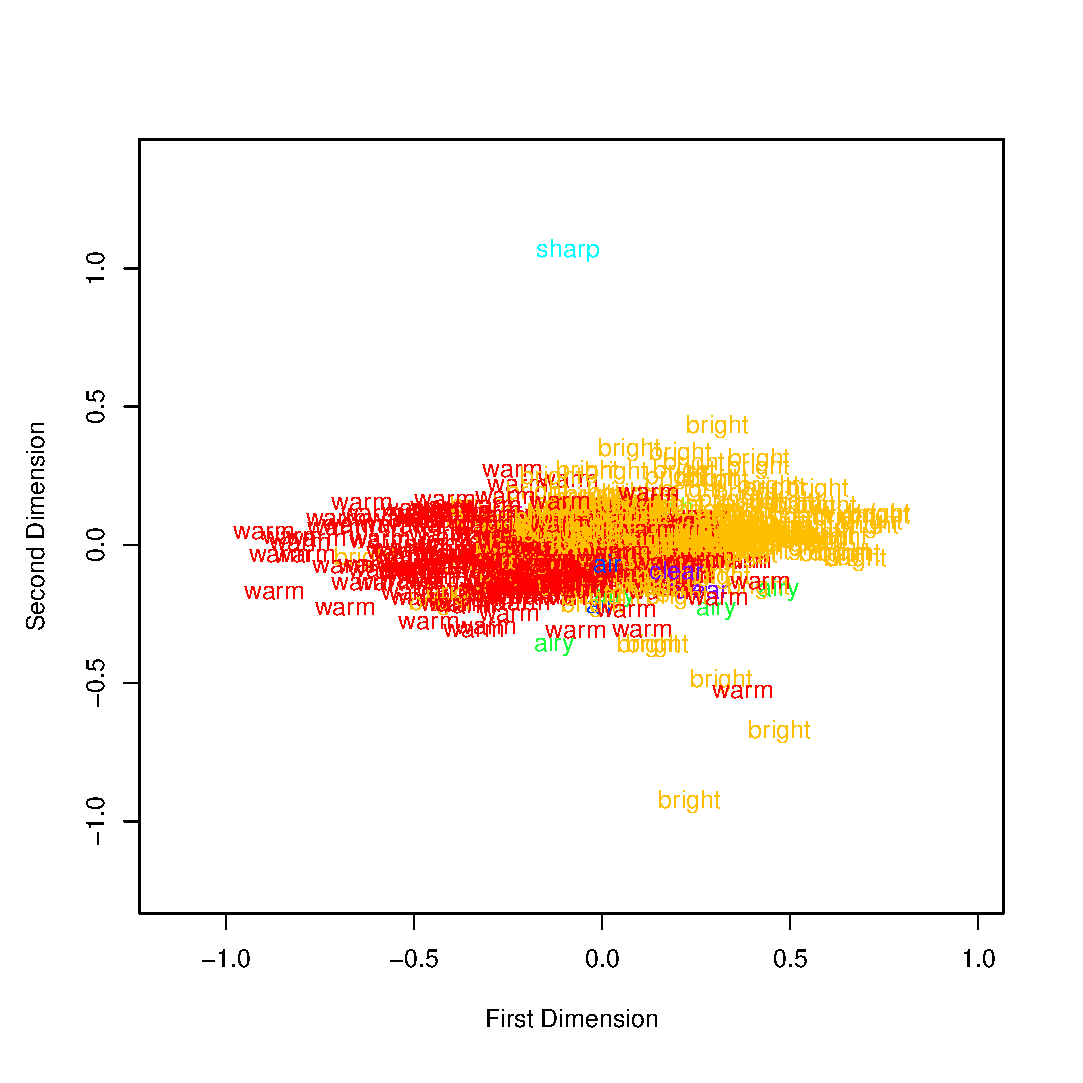
\includegraphics[width=0.45\textwidth]{chapter4/Images/EqualiserDifferenceMDS.eps}
				\label{fig:EqualiserDifferenceMDS}
			}
			\qquad
			\subfloat[Descriptor Centroids]
			{
				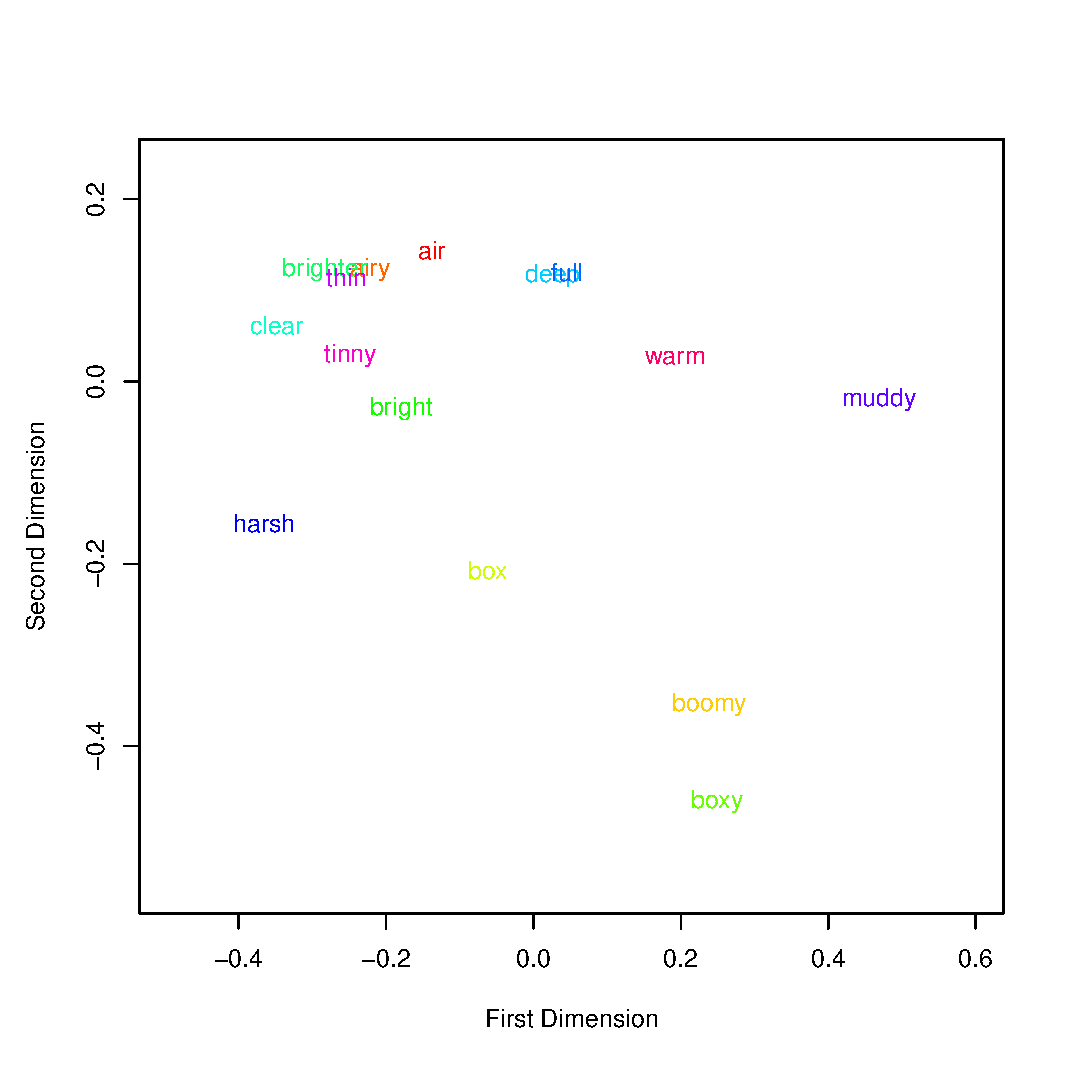
\includegraphics[width=0.45\textwidth]{chapter4/Images/EqualiserDifferenceCentroidsMDS.eps}
				\label{fig:EqualiserDifferenceCentroidsMDS}
			}
			\caption{Timbre Space for the Feature Differences from the Equaliser.}
			\label{fig:EqualiserDifferenceMDSs}
		\end{figure}

		\begin{table}[h!]
			\centering
			\begin{tabular}{|c|c|}
				\hline
				\bf{Feature} & \bf{Correlation} \\
				\hline
				\hline
				Peak Tristimulus 2 & 0.889 \\
				\hline
				Harmonic Tristimulus 2 & 0.884 \\
				\hline
				Noisiness & 0.884 \\
				\hline
				Harmonic Tristimulus 1 & 0.851 \\
				\hline
				Peak Tristimulus 1 & 0.849 \\
				\hline
				Fundamental & 0.811 \\
				\hline
			\end{tabular}
			\caption{Significant Features for Dimension 1 of the Timbre Spaces Shown in Figure 
				 \ref{fig:EqualiserDifferenceMDSs}.}
			\label{tab:EqualiserDifferenceFeaturesDim1}
		\end{table}

		\begin{table}[h!]
			\centering
			\begin{tabular}{|c|c|}
				\hline
				\bf{Feature} & \bf{Correlation} \\
				\hline
				\hline
				Irregularity K & -0.965 \\
				\hline
				Spectral Skewness & -0.936 \\
				\hline
				Peak Irregularity K & -0.930 \\
				\hline
				Spectral Kurtosis & -0.922 \\
				\hline
				Harmonic Irregularity K & -0.887 \\
				\hline
				Harmonic Spectral Kurtosis & -0.863 \\
				\hline
				Bark Coefficient 9 & -0.816 \\
				\hline
				Bark Coefficient 8 & -0.813 \\
				\hline
				Bark Coefficient 10 & -0.803 \\
				\hline
			\end{tabular}
			\caption{Significant Features for Dimension 2 of the Timbre Spaces Shown in Figure 
				 \ref{fig:EqualiserDifferenceMDSs}.}
			\label{tab:EqualiserDifferenceFeaturesDim2}
		\end{table}
